\section{Reverse-engineering the TRM circuit}
\label{sec:reverse}

Following Section~4 of \citet{nanda2023progress}, we reverse-engineer the grokked TRM by combining weight-level and activation-level evidence.

\subsection{Neuron-logit map $W_L$}
In the one-layer transformer, $W_L = W_U W_{\mathrm{out}}$ maps MLP neuron activations to logits.
For TRM SwiGLU blocks, the analogous map for layer $\ell$ is
$W_L^{(\ell)} = W_{\mathrm{down}}^{(\ell)} W_U^\top$.
We compute a 1D DFT of each row of $W_L$ along the logit axis and measure $\ell_2$ norm per frequency pair (Figure~\ref{fig:wl}).

At convergence, the final-layer $W_L$ peaks at frequencies $\BMIWLKeyFreqs$, aligning with progress-measure key frequencies $\BMIKeyFreqs$.

\begin{figure}[h]
  \centering
  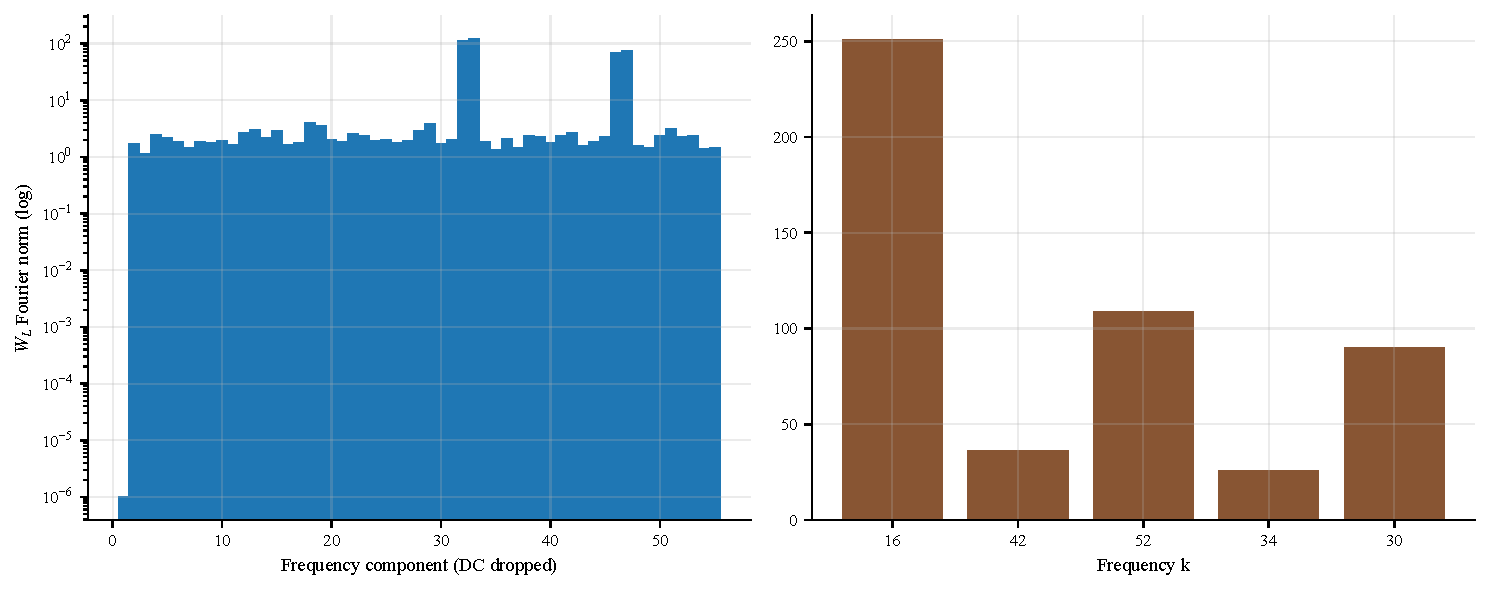
\includegraphics[width=0.95\linewidth]{figures/fig_wl_mlp_reverse_engineering.pdf}
  \caption{Left: $W_L$ Fourier norms on the final MLP layer. Right: neuron count per key frequency after clustering.}
  \label{fig:wl}
\end{figure}

\subsection{MLP neuron clustering}
We capture post-SwiGLU activations at the ``$=$'' token for all $(a,b)\in\{0,\ldots,P-1\}^2$ pairs.
Each neuron $n$ is assigned the frequency $k$ maximizing $R^2$ between its activation and $\cos(\omega_k(a+b))$ or $\sin(\omega_k(a+b))$.
The majority of neurons in the final layer align with one of the five key frequencies, consistent with the Fourier multiplication subcircuit.

\subsection{Attention routing}
Figure~\ref{fig:attn} shows mean attention from the ``$=$'' query position to tokens $a$, $b$, and ``$=$'' for each head in layer~0.
Post-grokking, heads route information from operand tokens into the output position, enabling the MLP to compute $\cos(\omega_k(a+b))$ and $\sin(\omega_k(a+b))$ via trigonometric identities.

\begin{figure}[h]
  \centering
  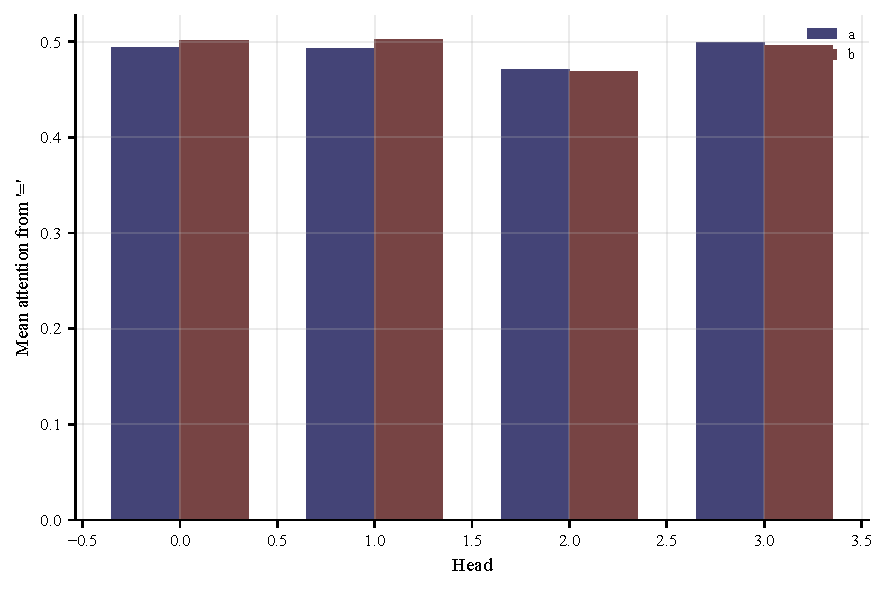
\includegraphics[width=0.7\linewidth]{figures/fig_attention_decomposition.pdf}
  \caption{Attention from ``$=$'' to $a$ and $b$ tokens (layer 0, per head).}
  \label{fig:attn}
\end{figure}

\subsection{Algorithm summary}
The TRM implements the same high-level algorithm as \citet{nanda2023progress}:
\begin{enumerate}
  \item \textbf{Embed} $a,b$ into sparse Fourier components via $W_E$.
  \item \textbf{Route} operand information to ``$=$'' via attention.
  \item \textbf{Compute} $\cos(\omega_k(a+b))$, $\sin(\omega_k(a+b))$ in SwiGLU neurons.
  \item \textbf{Unembed} to logits approximating $\cos(\omega_k(a+b-c))$ via $W_U$.
\end{enumerate}
Latent ACT recursion provides an additional guess channel (Section~\ref{sec:latent}) that becomes reliable only after the weight circuit forms.

\section{Latent recursion probes}
\label{sec:latent}

We adapt \citet{ren2026reasoning} to TRM's ACT outer loop.

\subsection{Reasoning modes}
On a 64-sample test batch at the final checkpoint, examples exhibit \textbf{trivial success}: correct prediction at ACT step~0 (Figure~\ref{fig:modes}).

\subsection{Fixed-point violation}
Fixed-point probes on the 20k-step final checkpoint show a violation rate of roughly $12.5\%$ on TRM-full variants (down from $\sim 78\%$ pre-grokking): the model can still corrupt previously correct outputs on later ACT steps despite near-perfect modular-addition accuracy.

\subsection{Latent trajectories}
PCA of $z_H$ at ``$=$'' across ACT steps (Figure~\ref{fig:pca}) shows curved trajectories rather than incremental refinement toward a stable attractor.

\begin{figure}[h]
  \centering
  
\includegraphics[width=0.95\linewidth]{figures/fig_latent_reasoning_modes.pdf}
  \caption{Mean-field CE along ACT steps and reasoning-mode counts (64 test samples).}
  \label{fig:modes}
\end{figure}

\begin{figure}[h]
  \centering
  
\includegraphics[width=0.6\linewidth]{figures/fig_latent_pca_trajectory.pdf}
  \caption{PCA of $z_H$ at ``$=$'' for one test example across ACT steps.}
  \label{fig:pca}
\end{figure}

\section{Multi-seed robustness}
\label{sec:multiseed}

We train $\BMINSeeds$ independent seeds for 50{,}000 steps with identical hyperparameters (Appendix~\ref{app:seeds}).
Figure~\ref{fig:multiseed} reports final test accuracy and grokking step (first step with test accuracy $>90\%$) per seed.
All seeds exhibit delayed generalization; key frequency sets vary slightly across seeds, as in Appendix~C.2 of \citet{nanda2023progress}.

\section{Related work}
Grokking was first characterized by \citet{power2022grokking}; \citet{nanda2023progress} provided the first mechanistic account via Fourier circuits on modular addition.
Latent and hierarchical models exhibit segment-wise grokking \citep{ren2026reasoning,jolicoeur2025less}.
Our work unifies these threads by measuring weight-level progress \emph{and} latent ACT probes in the same TRM training run.

\section{Limitations}
Under a data-driven key-frequency count, the Nanda baseline reaches faithful
trig-FVE $\HybridNandaFVEAdaptive$ (matching the $\sim$95\% of
\citet{nanda2023progress}) and the converged minimal-TRM seeds reach $\approx 0.99$;
the remaining minimal seeds and full TRM stay below this even with additional
frequencies, indicating a genuinely less sparse-Fourier logit map at convergence
rather than a measurement artifact.
We leave recursion-aware regularization and full attention-head circuit proofs to future work.
